\section{问题四：收缩移动边界的物质坐标模型}

\subsection{相对问题三的两处改动}

本问相对问题三改变了两件事：物性关系由式~\eqref{eq:prop_app3} 换成式~\eqref{eq:prop_app4}，
求解域由固定半径换成随时间收缩的 $r\in[0,R(t)]$。达标判据式~\eqref{eq:tend} 与插值定位
式~\eqref{eq:interp} 保持不变，边界条件式~\eqref{eq:bc_surface} 的形式不变但作用位置随
$R(t)$ 移动。两处改动中，物性只是系数替换，域的变化才是本质困难。

干基含水率 $C$ 以干物质质量为基准。药材收缩时，固体骨架携带结合水一起向内运动，
因此 $C$ 首先是物质点上的场，而不是实验室固定半径上的场。若仍在随时间缩小的物理网格上
离散，每步都要重新生成结点并把旧解插值过来，插值既破坏离散守恒，又使误差来源难以区分。
坐标变换的目的，就是把物质点变成固定的计算坐标。

\subsection{物质坐标与归一化坐标}

定义归一化物质坐标
\begin{equation}\label{eq:eta}
\eta=\bigl(r/R(t)\bigr)^2\in[0,1].
\end{equation}
均匀收缩假设下，固相速度为仿射场
\begin{equation}\label{eq:vs}
v_s(r,t)=r\,\dot R(t)/R(t),
\end{equation}
它是使 $\eta$ 对每个干物质质点保持不变的唯一径向速度，也使全局干物质
$S=\bar\rho_d(t)R(t)^2/2$ 在 $\bar\rho_d\propto R^{-2}$ 时守恒。
在定 $\eta$ 的物质导数下，前三问同一套经验扩散方程变为
\begin{equation}\label{eq:lagrange_C}
\frac{\partial C}{\partial t}
=\frac{4}{R(t)^2}\frac{\partial}{\partial\eta}\!\left(\eta\,D(C,T)\frac{\partial C}{\partial\eta}\right),
\end{equation}
能量方程同理，只把 $D$ 换成 $k$、左端乘 $\rho c_p$。收缩进入系数 $4/R^2$：半径缩小使同一
无量纲梯度对应更陡的物理梯度，扩散路径变短。方程中不再出现表观对流项，也无需再引入
开关参数 $\chi$。表面边界条件化为
\begin{equation}\label{eq:lagrange_bc}
\left.-\frac{2D}{R}\frac{\partial C}{\partial\eta}\right|_{\eta=1}=h_m\bigl[C(1,t)-C_{\rm air}\bigr],
\end{equation}
温度侧把 $D,h_m$ 换成 $k,h$。

为交叉验证，把同一经验方程写在实验室参考系后再作 Landau 变换 $\xi=r/R(t)$，
定 $\xi$ 求导与定 $r$ 求导相差 $-\xi\dot R/R\,\partial_\xi C$，计算域上多出一项表观对流。
该项来自坐标变形而不是真实流动；一阶迎风用以保证对角占优。两种坐标的关系见图~\ref{fig:landau_map}。
本文以物质坐标~\eqref{eq:lagrange_C} 为交付实现，以 Eulerian Landau（保留对流项）为交叉验证。

\begin{figure}[H]
  \centering
  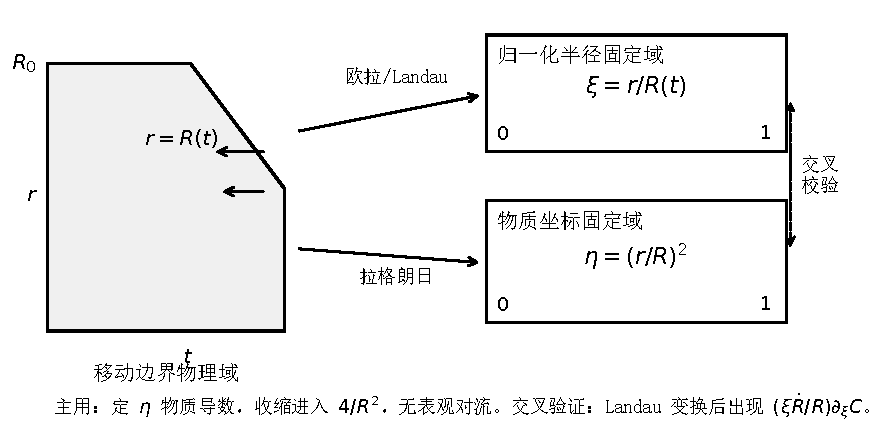
\includegraphics[width=0.92\textwidth,height=0.72\textheight,keepaspectratio]{../figures/tikz_landau_map.pdf}
  \caption{收缩物理域经物质坐标与 Landau 坐标映为固定计算域}
  \label{fig:landau_map}
\end{figure}

\subsection{半径时程}

式~\eqref{eq:lagrange_C} 需要 $R(t)$。附件 2 的 $145$ 个半径实测点全部参与插值：先按假设 5
作累积最小值以保证单调不增，再用保形分段三次插值构造连续曲线\upcite{Fritsch1980}。
半径由 $2.000$~cm 降至 $1.198$~cm，末态体积约为初始的 $36\%$。单调化前后的最大偏差为
$2.2\times10^{-16}$~cm，说明实测本身已经单调。$R(t)$ 与 $\dot R(t)$ 见图~\ref{fig:input_shrinkage}。

\begin{figure}[H]
  \centering
  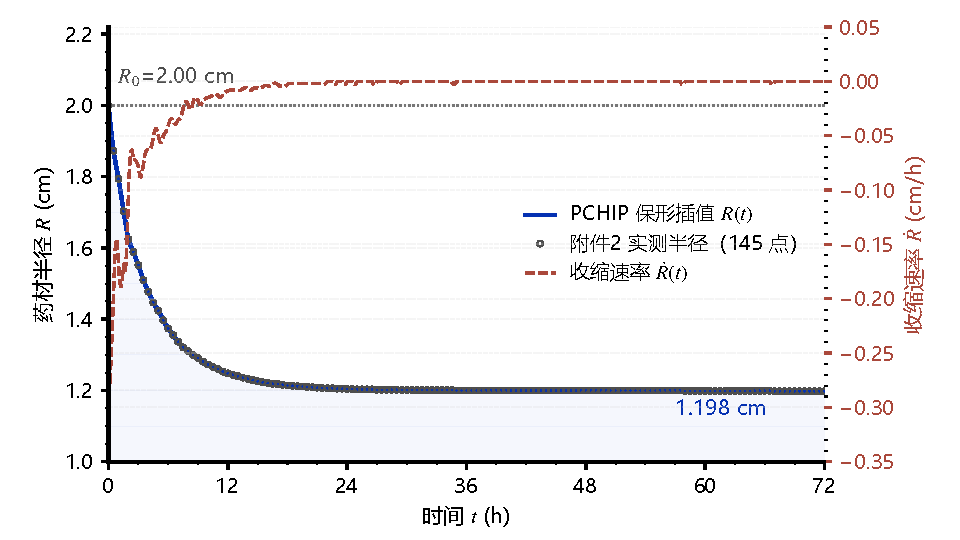
\includegraphics[width=0.9\textwidth,height=0.72\textheight,keepaspectratio]{../figures/fig_input_shrinkage.pdf}
  \caption{附件 2 收缩半径的实测散点、插值与收缩速率}
  \label{fig:input_shrinkage}
\end{figure}

\subsection{烘干时长与含水率分布}

物质坐标下求得烘干时长
\begin{equation}\label{eq:p4_answer}
t_{\rm end}=50.780~\mathrm{h}\approx 2.12~\mathrm{d}.
\end{equation}
该时刻逐点最大含水率为 $0.1500$~kg/kg，末态半径 $R(t_{\rm end})=1.20$~cm，落在附件 2
数据覆盖之内，不涉及外推。各时刻含水率分布见表~\ref{tab:p4_C}。

\begin{table}[H]
\centering
\caption{考虑收缩时药材内部水分浓度（kg/kg）}\label{tab:p4_C}
\begin{tabular}{ccccccc}
\toprule
时间 (h) $\backslash$ 距中心距离 (cm) & 0 & 0.5 & 1 & 1.5 & 2 & 药材表面 \\
\midrule
6  & 1.7165 & 1.5346 & 1.0212 & --- & --- & 0.4215 \\
12 & 0.7343 & 0.6516 & 0.4068 & --- & --- & 0.1666 \\
18 & 0.4067 & 0.3668 & 0.2387 & --- & --- & 0.0889 \\
24 & 0.2838 & 0.2598 & 0.1781 & --- & --- & 0.0671 \\
30 & 0.2253 & 0.2084 & 0.1485 & --- & --- & 0.0593 \\
36 & 0.1920 & 0.1789 & 0.1310 & --- & --- & 0.0558 \\
42 & 0.1705 & 0.1597 & 0.1194 & --- & --- & 0.0539 \\
48 & 0.1555 & 0.1462 & 0.1111 & --- & --- & 0.0528 \\
烘干结束时间 50.780 h & 0.1500 & 0.1412 & 0.1079 & --- & --- & 0.0525 \\
\bottomrule
\end{tabular}
\end{table}

$t=6$~h 时半径已缩至约 $1.37$~cm，$1.5$~cm 与 $2$~cm 两列自第一个输出时刻起即为空，
这是几何事实而不是缺算。同一套附录 4 物性、但半径冻结在 $2$~cm 时时长为 $128.906$~h，
引入收缩后缩短 $60.6\%$：收缩是主效应，不是小扰动。收缩域内的场演化见图~\ref{fig:q4_moving_boundary}。

\begin{figure}[H]
  \centering
  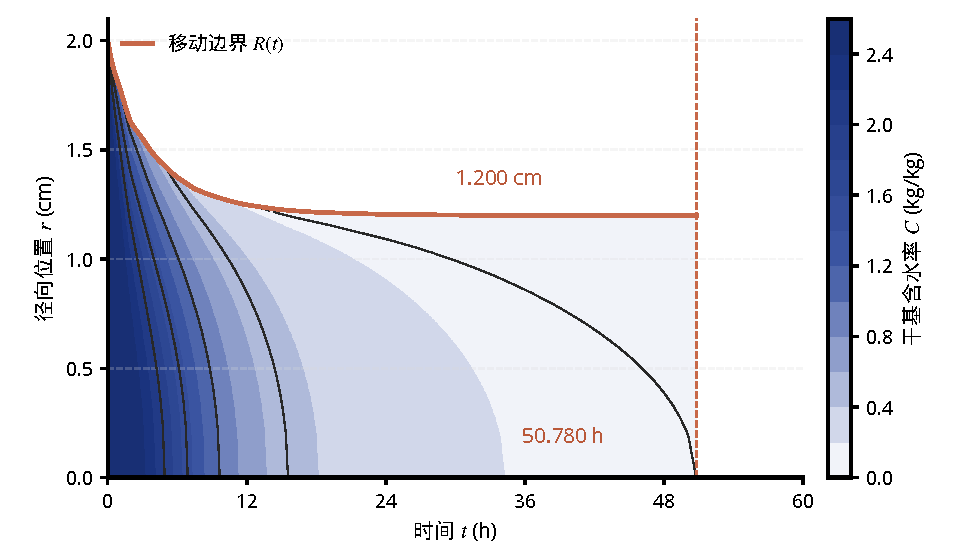
\includegraphics[width=0.9\textwidth,height=0.72\textheight,keepaspectratio]{../figures/fig_q4_moving_boundary.pdf}
  \caption{问题四收缩域内含水率的时空分布与移动边界}
  \label{fig:q4_moving_boundary}
\end{figure}

Eulerian Landau 交叉验证给出 $52.190$~h，与物质坐标结果相对相差 $2.78\%$。
相差来自是否让含水率随骨架一起运动，而不是来自网格重划。本文将
$[50.78,\,52.19]$~h 作为坐标表述带来的模型区间，交付值取物质坐标的 $50.780$~h。

\subsection{物性与收缩的 $2\times2$ 因子设计}

式~\eqref{eq:p4_answer} 比问题三的 $56.706$~h 短 $5.926$~h。但本问同时改了物性与求解域，
把净差说成「收缩使干燥加快」是混淆归因。在完全相同的离散、环境与判据下补齐四种组合，
见图~\ref{fig:effect_isolation} 与表~\ref{tab:effect}。

\begin{figure}[H]
  \centering
  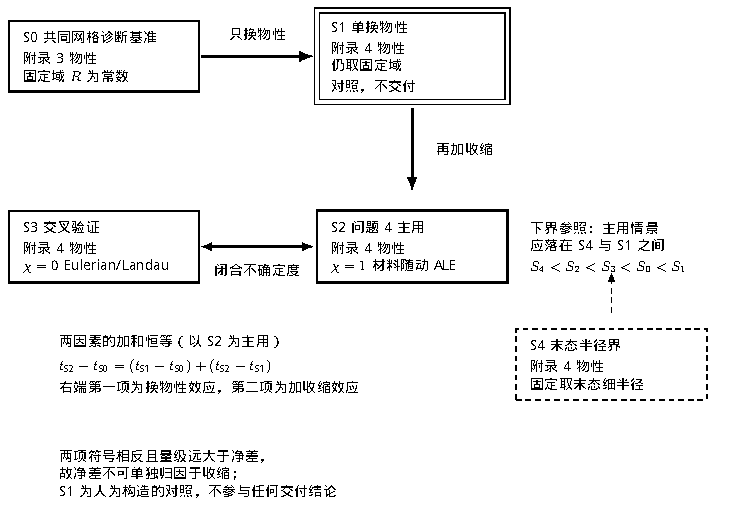
\includegraphics[width=0.95\textwidth,height=0.72\textheight,keepaspectratio]{../figures/tikz_effect_isolation.pdf}
  \caption{问题四相对问题三的 $2\times2$ 因子设计}
  \label{fig:effect_isolation}
\end{figure}

\begin{table}[H]
\centering
\caption{四种情景的烘干时长（Lagrangian 核）}\label{tab:effect}
\begin{tabular}{cllc}
\toprule
情景 & 物性关系 & 求解域 & $t_{\rm end}$ (h) \\
\midrule
$t_{00}$ & 附录 3 & 固定 $R=2$~cm & 56.974 \\
$t_{10}$ & 附录 4 & 固定 $R=2$~cm（对照） & 128.906 \\
$t_{01}$ & 附录 3 & 收缩 $R(t)$ & 25.088 \\
$t_{11}$ & 附录 4 & 收缩 $R(t)$（交付） & 50.780 \\
\bottomrule
\end{tabular}
\end{table}

非线性系统中，两因素的贡献依赖计算路径。先换物性再加收缩，得
$+71.932$~h 与 $-78.126$~h；先加收缩再换物性，得 $-31.886$~h 与 $+25.692$~h。
交互项
\begin{equation}\label{eq:interaction}
I=t_{11}-t_{10}-t_{01}+t_{00}=-46.240~\mathrm{h}
\end{equation}
与主效应同量级，说明加性分解不是唯一因果分解——这正是 $t\sim R^2/D$ 的乘积结构所预期的。
若仍需报两个单一贡献，取两条路径的平均（Shapley）
\begin{equation}\label{eq:shapley}
\Delta_{\rm prop}=+48.812~\mathrm{h},\qquad
\Delta_{\rm shrink}=-55.006~\mathrm{h},\qquad
\Delta_{\rm net}=-6.194~\mathrm{h}.
\end{equation}
机器精度下的加和残差只说明算术闭合，不能证明分解可靠，本文不再把它当作验证指标。
四格时长的对照见图~\ref{fig:q4_shrink_effect}。

\begin{figure}[H]
  \centering
  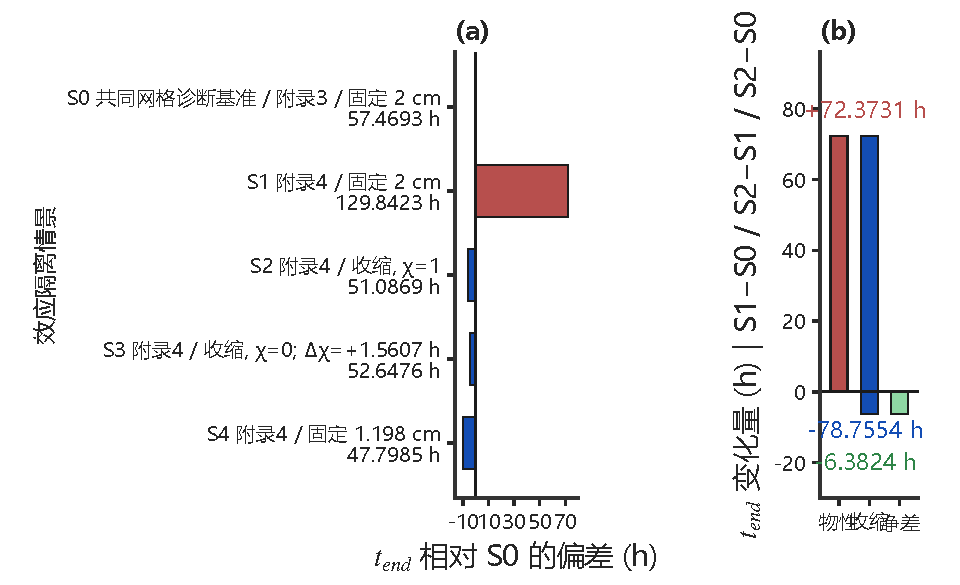
\includegraphics[width=0.95\textwidth,height=0.72\textheight,keepaspectratio]{../figures/fig_q4_shrink_effect.pdf}
  \caption{问题四 $2\times2$ 因子设计与两条路径的贡献}
  \label{fig:q4_shrink_effect}
\end{figure}

$t_{01}=25.088$~h 说明：若仍用附录 3 的较快扩散、同时又允许收缩，时长会比问题三再短一半以上。
附录 4 的低扩散把这份加速部分抵消，最终交付值落在 $50.780$~h。Eulerian 四格给出几乎同一
交互项（$I=-45.468$~h），结论不依赖于坐标选择。

物质坐标与 Eulerian 的逐点最大含水率对照见图~\ref{fig:chi_closure}。

\begin{figure}[H]
  \centering
  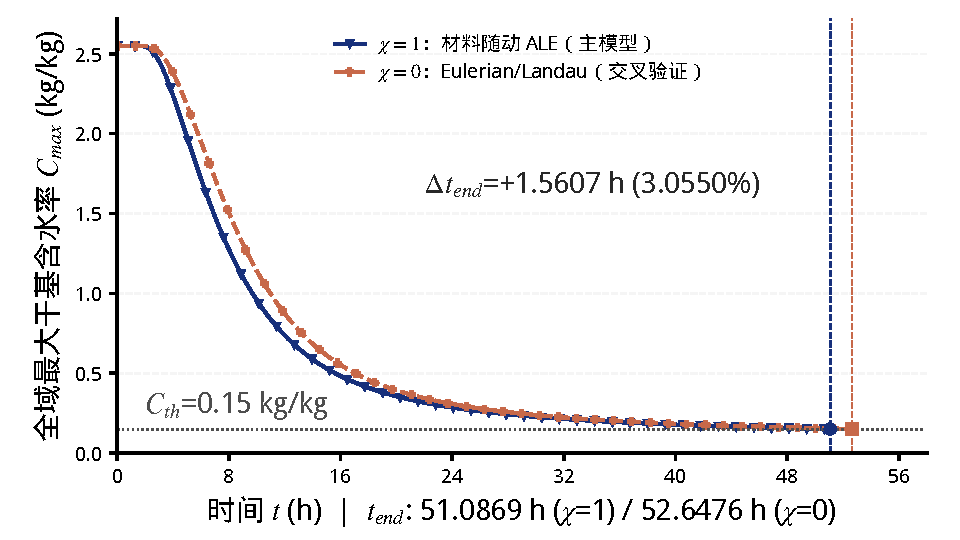
\includegraphics[width=0.88\textwidth,height=0.72\textheight,keepaspectratio]{../figures/fig_chi_closure.pdf}
  \caption{物质坐标与 Eulerian Landau 的交叉验证}
  \label{fig:chi_closure}
\end{figure}

\subsection{收缩律与数据自洽性}

由附件 2 的 $R(t)$ 与干基质量加权平均含水率 $\bar C(t)$ 反演体积收缩系数
$\beta(t)=\bigl[(R/R_0)^2-1\bigr]/(\bar C-C_0)$。若线性收缩律成立，$\beta$ 应为常数；
实际 $\beta$ 的均值为 $0.298$、变异系数 $22\%$，线性收缩律不成立。因此本文直接使用实测
$R(t)$，而不把体积写成 $C$ 的仿射函数。

最后报告题给数据本身的不相容。若干物质守恒，则 $\rho_s(C_{\rm th})/\rho_s(C_0)=(R_0/R_{\rm end})^2$。
按式~\eqref{eq:prop_app4} 左端为 $2.413$、附件 2 右端为 $2.787$，相差 $13.42\%$；
由密度反演的末态半径为 $1.287$~cm，实测为 $1.198$~cm。题目要求根据附件 2 确定时长，
故把实测 $R(t)$ 作为给定移动边界，不相容度只作诊断，既不修正半径，也不当作收敛判据。
该不一致对时长的影响不能用坐标交叉验证的 $2.78\%$ 去代替，必须另算；本文未把这一项
并入交付不确定度区间。诊断见图~\ref{fig:q4_mass_consistency}。

\begin{figure}[H]
  \centering
  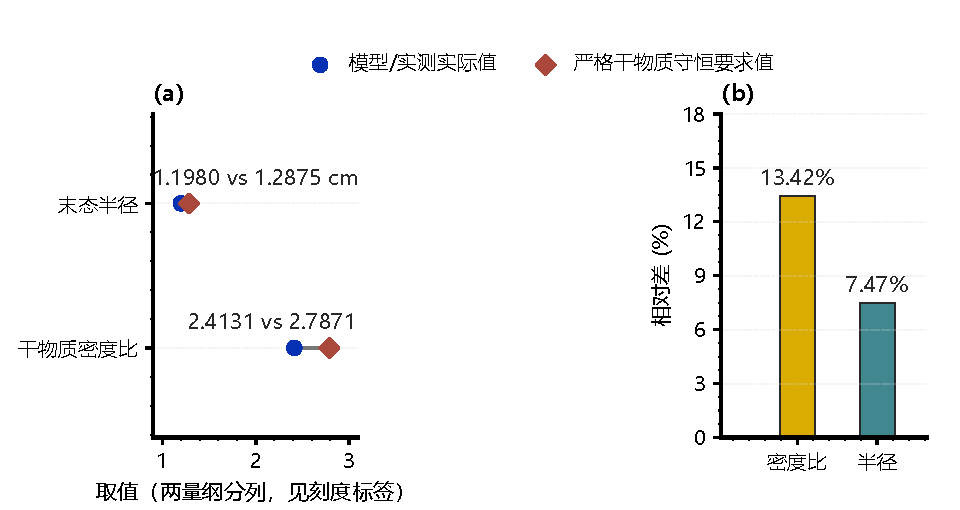
\includegraphics[width=0.88\textwidth,height=0.72\textheight,keepaspectratio]{../figures/fig_q4_mass_consistency.pdf}
  \caption{附录 4 密度关系与附件 2 收缩数据的干物质自洽性诊断}
  \label{fig:q4_mass_consistency}
\end{figure}
